\section{Problem Formulation}\label{sec:problem_definition}
Let $S$ denote a set of subjects of potential interests to journalists. 
For example, $S$ can refer to all the players or teams in the NBA application.
%In this paper, we consider the news themes generated from an aggregate function a single attribute of events.
%Extending our method to consider news themes on different attribute is straightforward.
%
%
%Take the NBA application as an example, we can build a news theme detector on the ``point'' attribute of the players to automatically generate newsworthy themes. To cover all the attributes of the players, we can deploy multiple news detectors on each attribute with different user defined aggregation functions.
Let $e_s(t)$ denote an event about subject $s$, where $t$ denotes its timestamp or sequence ID. For example, an event can refer to an NBA game a player participated on a certain day. Note that we maintain a sequence ID for each subject that is automatically incremented. It is possible that the events of different subjects may have the same sequence IDs. A sequence of consecutive events of the same subject is grouped as an \textit{event window}:

%%%TAN:i don't think incremental is the right word. suggest changing to:
%maintain a sequence ID for each subject that is automatically incremented.

\begin{definition}[Event Window]
Let $w$ be a window length, an event window $W_s(t,w)$ refers to $w$ consecutive events of subject $s$ and ending at sequence $t$, i.e., $W_s(t,w)=\{e_s(t-w+1),..., e_s(t)\}$.
\end{definition}

In general, if a subject $s$ has $|\mathbb{H}_s|$ events, there are $|\mathbb{H}_s|\choose{2}$ possible event windows. Given an aggregate function $f$, events in an event window can be aggregated to a numerical value $\overline{v}$ as:
$$W_s(t,w).\overline{v} = f(e_s(t-w+1),..., e_s(t))$$

We support all the common aggregate functions such as \emph{sum}, \emph{avg}, \emph{count}, \emph{min} and \emph{max}. 
For simplicity of presentation, we only consider a single aggregate function in our solution. To support multiple aggregation functions, one may simply invoke our solution multiple times to process them independently.

\begin{example}
Fig.~\ref{fig:system_flow} (A) illustrates examples of \textit{event window}s of three NBA players. 
Each event represents the points scored by a player in a game. 
In the figure, the event window $W_{s_1}(3,2)$ refers to two consecutive events about player $s_1$ ending at $t=3$, i.e., $W_{s_1}(3,2)=\{e_{s_1}(2), e_{s_1}(3)\}$. Given an aggregate function $f=avg(points)$,  we yield $W_{s_1}(3,2).\overline{v}=(46+10)/2=28$.
\end{example}

\begin{figure*}[t]
\centering
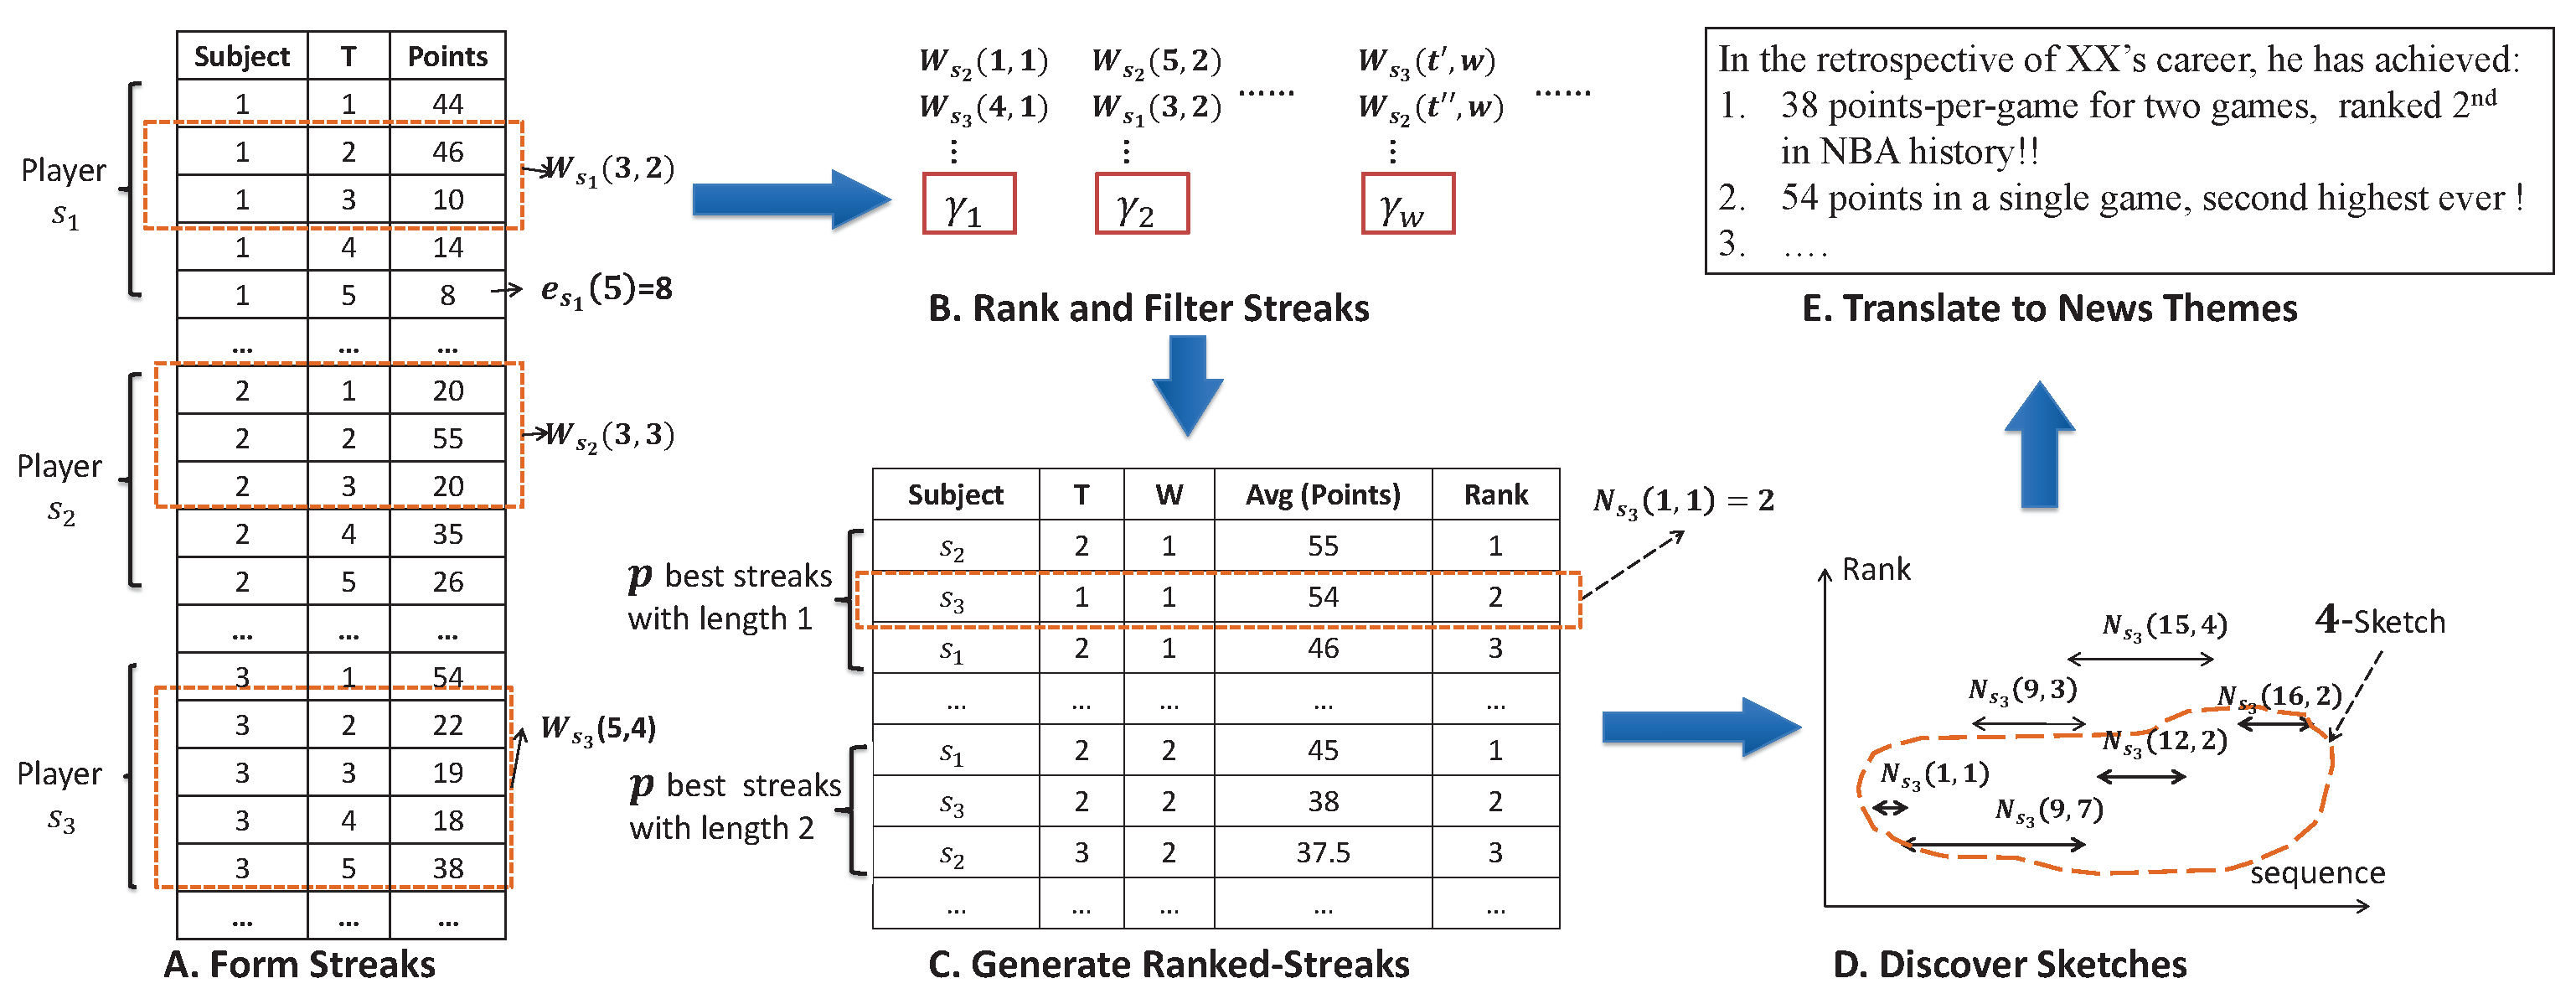
\includegraphics[width=1.0\textwidth]{chapter4/charts/application.eps}
	\caption{An illustration sketch discovery workflow. 
(A): various event windows are formed based on events' sequence IDs. 
(B): event windows with rank greater than $p$ are filtered.
(C): best ranked event windows form candidate themes.
(D): $k$-sketches are discovered for each subject from their candidate themes.
(E): subject related news can be generated from each $k$-sketch.
}
\label{fig:system_flow}
\end{figure*}

With the aggregated value $\overline{v}$, we can derive the rank of an event window, which can be used to measure the strikingness of an event window as a news theme.  For instance, ``\textit{The total points Kobe has scored is $32,482$}'' can be transformed into a rank-aware representation: ``\textit{Kobe moved into third place on the NBA's all-time scoring list}'', in which the rank is $3$. Let $W$ be a length-$w$ event window, and 
 $\gamma_w(W.\overline{v})$ be the rank of $W$ by comparing it with all other
length-$w$ event windows on their aggregate values. Generally speaking, an event window is newsworthy if its rank is smaller than a predefined threshold. This leads to our definition of \emph{Candidate Theme}:
%

\begin{definition} [Candidate Theme]
An event window $W_s(t,w)$ is said to be a candidate theme, denoted by $N_s(t,w)$, if its rank $\gamma_w(W_s(t,w).\overline{v}) \leq p$. $p$ is a user-defined threshold.

%which is a triple $\langle t, w, \gamma_w(W_s(t,w).\overline{v})\rangle$.
\end{definition} 

\begin{example}
In the step $(B)$ of Fig.~\ref{fig:system_flow}, we group the event windows based on their window length. Each window is associated with a rank value $\gamma_w$. If the rank value is greater than the threshold $p$, the associated event window is pruned. Otherwise, it is considered as a candidate. In the step $(C)$ of  Fig.~\ref{fig:system_flow}, we present the candidate themes  in the tabular format. Each candidate contains the rank computed from step (B). For instance, among all candidate themes with window length 1, $N_{s_3}(1,1)$ (with value $54$) is ranked 2nd because its aggregated value is smaller than that of another event window $N_{s_2}(2,1)$ (with value $55$). %Therefore the rank of $N_{s_3}(1,1).\gamma=2$.
\end{example}

Let $\mathbb{N}_s$ be the set of candidate themes of subject $s$. Since for each possible window length, there are at most $p$ candidate themes, the size of $\mathbb{N}_s$ can be as large as $p|\mathbb{H}_s|$, which is still overwhelming for news reporting.
To control the output size while maintaining the quality of news themes, we
aim to find, for each subject $s$, a small subset of $k$ 
candidate themes from $\mathbb{N}_s$. %, which $best$ describes $\mathbb{N}_s$. 
We call the subset  a $k$-\textbf{Sketch}. 

To measure the quality of a sketch, we define a scoring 
function $g(\cdot)$ over all sketches. The design of $g$ gives rise to two concerns.
First, $g$ needs to assign higher scores to the candidate themes with better ranks. This
is because better rank indicates good strikingness which implies that the news theme would
be more eye-catching. For instance, 
we can expect people to care more about who the top scorer in NBA history is rather than who ranked 20$^{th}$ in the history.
Second, $g$ prefers the sketches containing candidate themes with fewer overlapped events and avoids near-duplicate events. 
This is because near-duplicate themes generally do not add news values.
For example, when Kobe Bryant scored 81 points in a single game (2nd highest in NBA history),
all event windows containing that event are likely to have good and similar ranks. 
Thus, reporting all of them is not newsworthy.

To resolve these two concerns, we define $g$ as follows: given any set $\mathbb{X}_s$
of candidate themes about subject $s$ (i.e., $\mathbb{X}_s \subseteq \mathbb{N}_s$), 
the score of $\mathbb{X}_s $ is:
\begin{equation}
	\label{eq:scoring_function}
	g (\mathbb{X}_s) = \alpha C(\mathbb{X}_s) + (1-\alpha) R(\mathbb{X}_s), \alpha \in [0,1]
\end{equation}
where $C(\mathbb{X}_s)$ is the ratio between the number of distinct events covered by $\mathbb{X}_s$ 
over the total number of events about subject $s$. In this way, duplicated candidate themes 
contribute to a lower score. $R(\mathbb{X}_s) = \frac{1}{|\mathbb{X}_s|}\sum_{X_s \in \mathbb{X}_s} \frac{p-X_s.\gamma}{p}$ is the strikingness of $\mathbb{X}_s$. Any candidate themes in 
$\mathbb{X}_s$ changing to a better rank increases $R(\mathbb{X}_s)$. The values of $C(\mathbb{X}_s)$ and $R(\mathbb{X}_s)$ are normalized  between $[0,1]$. $\alpha$ is an adjustable coefficient to balance the weights between $C(\mathbb{X}_s)$ and $R(\mathbb{X}_s)$. If $\alpha$ is high, it means users are more interested in finding news themes that cover most of the subject's events.  If $\alpha$ is low, it indicates users prefer news themes whose ranks are small. 

With Equation~\ref{eq:scoring_function}, we then define the \emph{Sketch Discovery} problem as follows:

\begin{definition} [Sketch Discovery]
Given a parameter $k$, Sketch Discovery aims to, for each subject $s$, 
find a subset $SK_s$ from the candidate themes of $s$ (i.e., $SK_s \subseteq \mathbb{N}_s$), s.t. $|SK|_s = k$ and $g(SK_s)$ is maximized.
\end{definition}

\begin{example}  
In the step (D) of Fig.~\ref{fig:system_flow}, we show a collection of candidate themes and a $k$-sketch derived from them. The y-axis is the rank and the x-axis represents the complete sequence of events of a subject. Each candidate theme is represented by a line segment, covering a window of events. When $k=4$, four of the candidate themes are selected as a $4$-sketch as the most representative news for the subject.	
\end{example}

Before we move on to the algorithmic part, we first list the notations in Table~\ref{tbl:notations}. For the 
ease of presentation, we present our techniques using \emph{avg} as the default aggregate function in the following sections. Extending our techniques to other aggregate functions will be addressed in Section~\ref{sec:discussion}.

\begin{table}[h]
\centering
\begin{tabular}{|c|l|}
\hline 
\textbf{Notation} & \textbf{Meaning} \\ 
\hline
$S$ & set of subjects \\
\hline
$\mathbb{H}_s$ & set of events associated with subject $s$\\
\hline
$W_s(t,w)$ & length-$w$ event window of $s$ ending at $t$\\
\hline
$\mathbb{N}_s$ & set of candidate themes associated with subject $s$\\
\hline 
$N_s(t, w)$ & candidate theme derived from $W_s(t,w)$ \\ 
\hline 
$WI(w)$ & $p$ best ranked candidate themes of window length $w$\\
\hline
$\beta(w)$ & lower bound of $WI(w)$\\
\hline
$SK_s$ & sketch for subject $s$ \\
\hline
$J_s$ & visiting-window bound for subject $s$ \\
\hline
$M_s$ & unseen-window bound for subject $s$\\
\hline
$P_s$ & online-window bound for subject $s$\\
\hline
\end{tabular} 
\caption{Notations used in this paper}
\label{tbl:notations}
\end{table}
